\chapter{Results of Workflow Validation}\label{chap:results}
The Galaxy workflows are validated using real-world datasets from different laboratories. The analysis results for each workflow with complying test samples are described below.

\section{Poxvirus Workflow with Lumpy Skin Disease Virus Datasets}
We employed our pipeline using a tiling amplicon approach with masked reference sequences for each half genome. Two public \ac{LSDV} samples, 20L70 (SRR15145276 and SRR15145275) and 20L81 (SRR15145274 and SRR15145273), that were sequenced with the required tiled amplicon method in two pools are used. Collected from cattle in 2020 during a lumpy skin disease outbreak in Northern Vietnam (20L70\_Dinh-To/VNM/20 and 20L81\_Bang-Thanh/VNM/20), both samples were sequenced on an MiSeq System using a NexteraXT. The used \acs{CaPV} primer scheme in \ac{BED} format contains pool identifier in the \textit{SCORE} column. The widely-used vaccine ``Neethling'' strain was used as reference genome (NC\_003027.1). The raw FASTQ files for each sample were trimmed with \texttt{fastp} and mapped to each half-masked reference.

\setlength{\tabcolsep}{16pt}
\renewcommand{\arraystretch}{1.3}
\begin{table}[ht!]
    \centering
    \begin{tabular}{lcc}
    \toprule
    \textbf{Output Metric}                      & \textbf{20L70}     & \textbf{20L81}     \\ \midrule
    Paired-end raw reads                        & 863 820            & 1 016 168          \\ 
    Paired-end reads after quality trimming     & 856 138            & 947 064            \\ \midrule
    Proportion of reads mapping to reference    & 99.6\%             & 77.3\%             \\ 
    Proportion of reference covered             & 99.68\%            & 99.68\%            \\ \midrule
    Mean coverage                               & 2 705.2 \texttimes & 2 411.4 \texttimes \\ 
    Alignment error rate                        & 1.25\%             & 1.30\%             \\ \bottomrule
    \end{tabular}
    \caption{Metrics after preprocessing and mapping for datasets 20L70 and 20L81.}
    \label{tab:4-pox-metrics}
\end{table}

The used primer scheme contains a total of 23 primers, while the first 12 primers cover \textit{pool1} and the remaining 11 primers cover \textit{pool2}. It was designed for the tiling amplicon approach and allows to generate the complete genome of all three members of Capripoxviruses, which includes the \ac{LSDV} sample. The primer scheme works with all Capripoxviruses due to the serological similarity they have. The primer scheme is provided in the Galaxy history of the test runs and is available via links in Supplementary~\secref{sec:apx-pox-links}. Inspection of the masking intervals for N-masking the reference confirms that the right-most position of Ns of masking the first half (i.e. preparing the reference for mapping \textit{pool2} reads) is the minimal start position of \textit{pool2} primers (``1 -- 79081'', and 79081 being the start position of primer 13). Accordingly for N-masking the reference for mapping of \textit{pool1} reads, the interval from the right-most primer-end of \textit{pool1} primers is 80202, the end position of primer 12, resulting in the interval ``80202 -- 150773''. The final position is the maximal end position and the total length of the reference sequence. Since the reference genome and primer scheme are the same for both datasets 20L70 and 20L81, the N-masked references are used for both mappings. Mapping of each pool is done with \texttt{BWA-MEM} and default settings for Illumina-sequenced reads, using the N-masked reference for \textit{pool1} and \textit{pool2} respectively. After merging the mappings with \texttt{Samtools merge}, statistics for preprocessing and mapping are reported and summarised in~\tabref{tab:4-pox-metrics}. \\
The merged mapping of both read pools is quality trimmed with \texttt{iVar trim} to remove primers and reads with a length of less than 30. The remaining reads are used for full-length consensus sequence construction with \textit{iVar consensus}, developed for amplicon-based sequencing data. Inspection of the consensus sequences for both samples shows that apart from the front and tail until the first and last primer positions a consensus sequence was produced and a base at each position could be found. \todo{consensus evaluation: \# of variants with respect to the reference genome (missense variants?)}

20L70: first 264/ last 269 positions N \\
20L81: first 264/ last 268 positions N


\section{AIV Workflow with H4N6 and H5N8 Samples}\label{sec:4-aiv}
The \ac{AIV} Illumina workflow on the Galaxy platform was evaluated using two field isolates provided by the Belgian Sciensano lab. The isolates were extracted in Belgium in 2020 from an H4N6 infected magpie (EPI\_ISL\_7593059) and an H5N8 infected duck (EPI\_ISL\_7596571). The samples were sequenced on an Illumina platform in paired-end mode and are utilised one sample per workflow run. For the \ac{AIV} Illumina workflow, a reference database in FASTA format is required as a collection with eight datasets, one per \ac{AIV} segment, which is uploaded in Galaxy. The database we used contains multiple sequences per segment as described in~\secref{sec:3-aiv-ref}. Although it misses very few subtypes that rarely occur, the variation within each subtype is generally captured well with the given database. Due to the filtering criteria, not all complete genome sequences were found suitable for the database.
\\

\setlength{\tabcolsep}{14pt}
\renewcommand{\arraystretch}{1.3}
\begin{table}[ht!]
    \begin{tabular}{lcc} 
    \toprule
    \textbf{Output Metric}                                                                & \textbf{EPI\_ISL\_7593059} & \textbf{EPI\_ISL\_7596571} \\ \midrule
    Paired-end raw reads                                                                  & 1 537 722                  & 858 610                    \\ 
    \begin{tabular}[c]{@{}l@{}}Paired-end reads after quality\\trimming\end{tabular}      & 1 507 396                  & 830 176                    \\ \midrule
    \end{tabular}
    \caption{Metrics after preprocessing of EPI\_ISL\_7593059 and EPI\_ISL\_7596571.}
    \label{tab:4-aiv-metrics}
\end{table}

After starting the workflow with one sample each, the paired-end reads are preprocessed and serve as query reads for \texttt{VAPOR}. Metrics are shown in~\tabref{tab:4-aiv-metrics}. Since the reference database contains eight FASTA files in a collection, the tool runs once per segment and outputs the highest scoring sequences per segment, which represents the most similar sequences from the database to the query sequence. 

\setlength{\tabcolsep}{8pt}
\renewcommand{\arraystretch}{1.3}
\begin{table}[]
    \centering
    \begin{tabular}{@{}llll@{}}
    \toprule
    \textbf{Segment} & \textbf{\begin{tabular}[c]{@{}l@{}}\% of query bases\\in reads\end{tabular}} & \textbf{Mean score} & \textbf{Subtype of hit} \\ \midrule
    % PB2         & 0.990 / 0.999                               & 9 013.9 / 8 951.4               & H12N5 / H5N8                      \\
    % PB1         & 0.981 / 0.997                               & 2 450.3 / 5 493.4               & H3N8 / H5N8                      \\
    % PA          & 0.994 / 1.0                               & 18 271.1 / 16461.2               & H1N1 / H5N8                      \\
    HA & 0.987 / 1.0 \textsuperscript{1}                      & 8 223.1 / 19 426.8      & H4N6 / H5N8             \\
    % NP          & 0.996 / 1.0                               & 26 427.3 / 12 250.9               & H7N3 / H5N8                      \\
    NA & 0.987 / 1.0                                         & 36 908.4 / 3 743.4      & H4N6 / H5N8             \\
    % M1          & 0.997 / 0.998                               & 50 202.7 / 17 034.3               & H1N1 / H5N8                      \\
    % NS1         & 1.0 / 1.0                               & 82 958.0 / 24 647.4               & H3N8 / H5N8                      \\
    \bottomrule
    \multicolumn{3}{l}{\textsuperscript{1} Results for EPI\_ISL\_7593059 / EPI\_ISL\_7596571}
    \end{tabular}
    \caption{The best scoring sequence of the VAPOR run for the AIV test samples.}
\label{tab:4-aiv-vapor}
\end{table}

The \texttt{VAPOR} search was able to successfully identify the avian influenza virus subtypes present in each sample: for the H5N8 sample, the most similar sequence of HA segment origins from a sample with the H5 subtype, while the most similar sequence of the NA segment origins from a sample with the N8 subtype. Similarly, the H4N6 sample was correctly identified. The results of the \texttt{VAPOR} run for the HA and NA genes are summarised in~\tabref{tab:4-aiv-vapor}.

S8: \\
H5N8 sample: HA gene: 1 SNP compared to reference sequence chosen by VAPOR (MZ166252) at position 1002 \\
H5N8 sample: NA gene: 1 SNP compared to reference sequence chosen by VAPOR (MZ166270) at position 497

S4: \\
H4N6 sample: HA gene: 30 SNPs compared to reference sequence chosen by VAPOR (LC121412) at positions xyz \\
H4N6 sample: NA gene: 29 SNPs compared to reference sequence chosen by VAPOR (MW419994) at positions xyz (there are better)

\todo{consensus sequence (no Ns), IQ-Trees for \ac{HA}/\ac{NA}}


\begin{figure}
\centering
    \begin{subfigure}[b]{1.1\textwidth}
        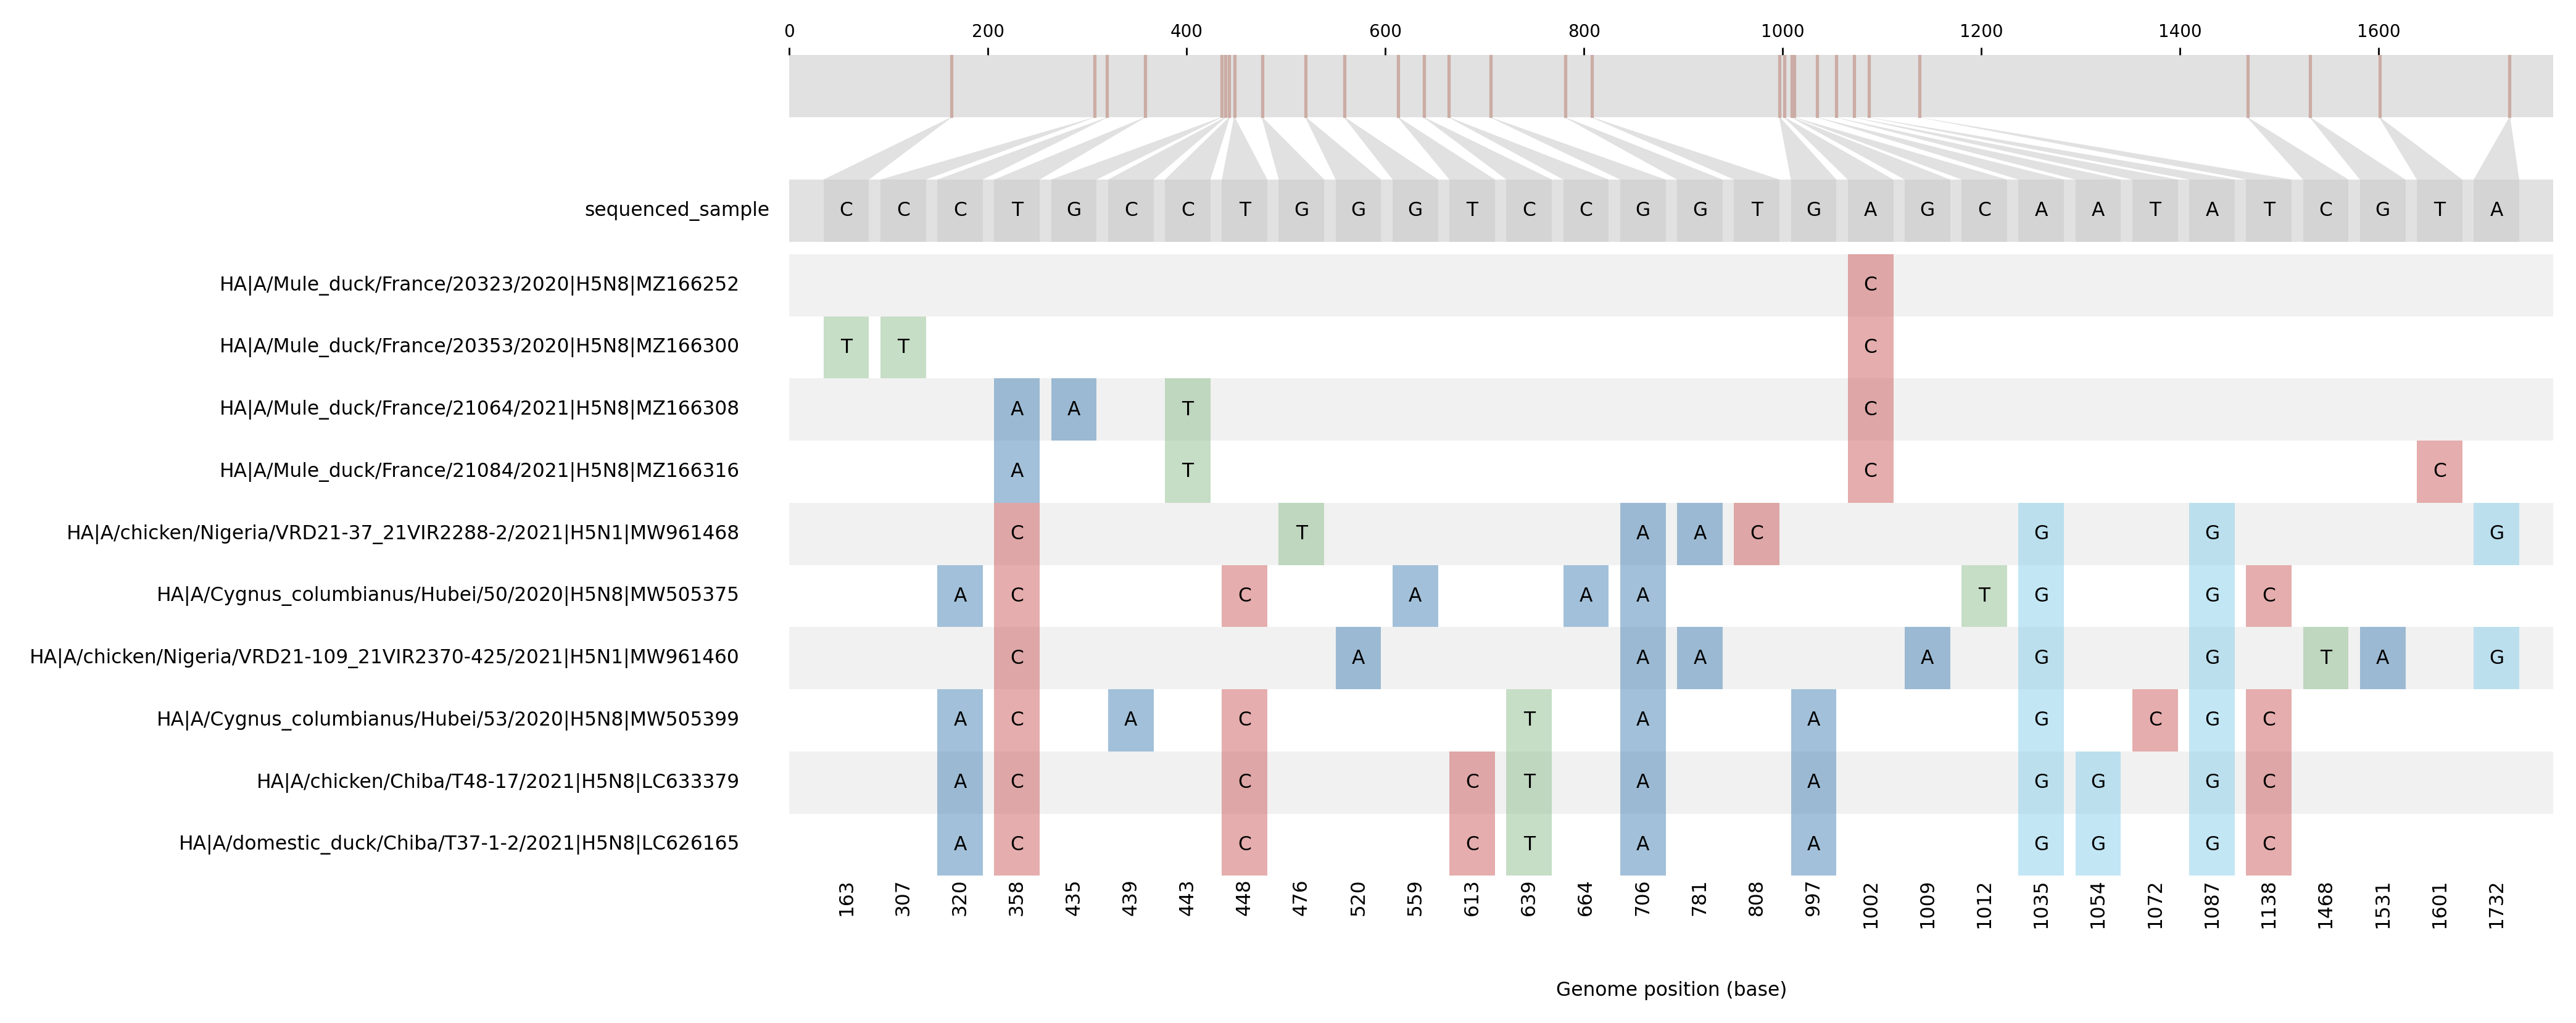
\includegraphics[width=1.0\linewidth]{media/4-aiv-snipit-s8-4-ha.png}
        \caption{SNPs of HA gene of H5N8 sample.}
    \label{fig:4-aiv-snipit-s8-ha}
    \end{subfigure}
    \\
    \begin{subfigure}[b]{1.1\textwidth}
        \centering
        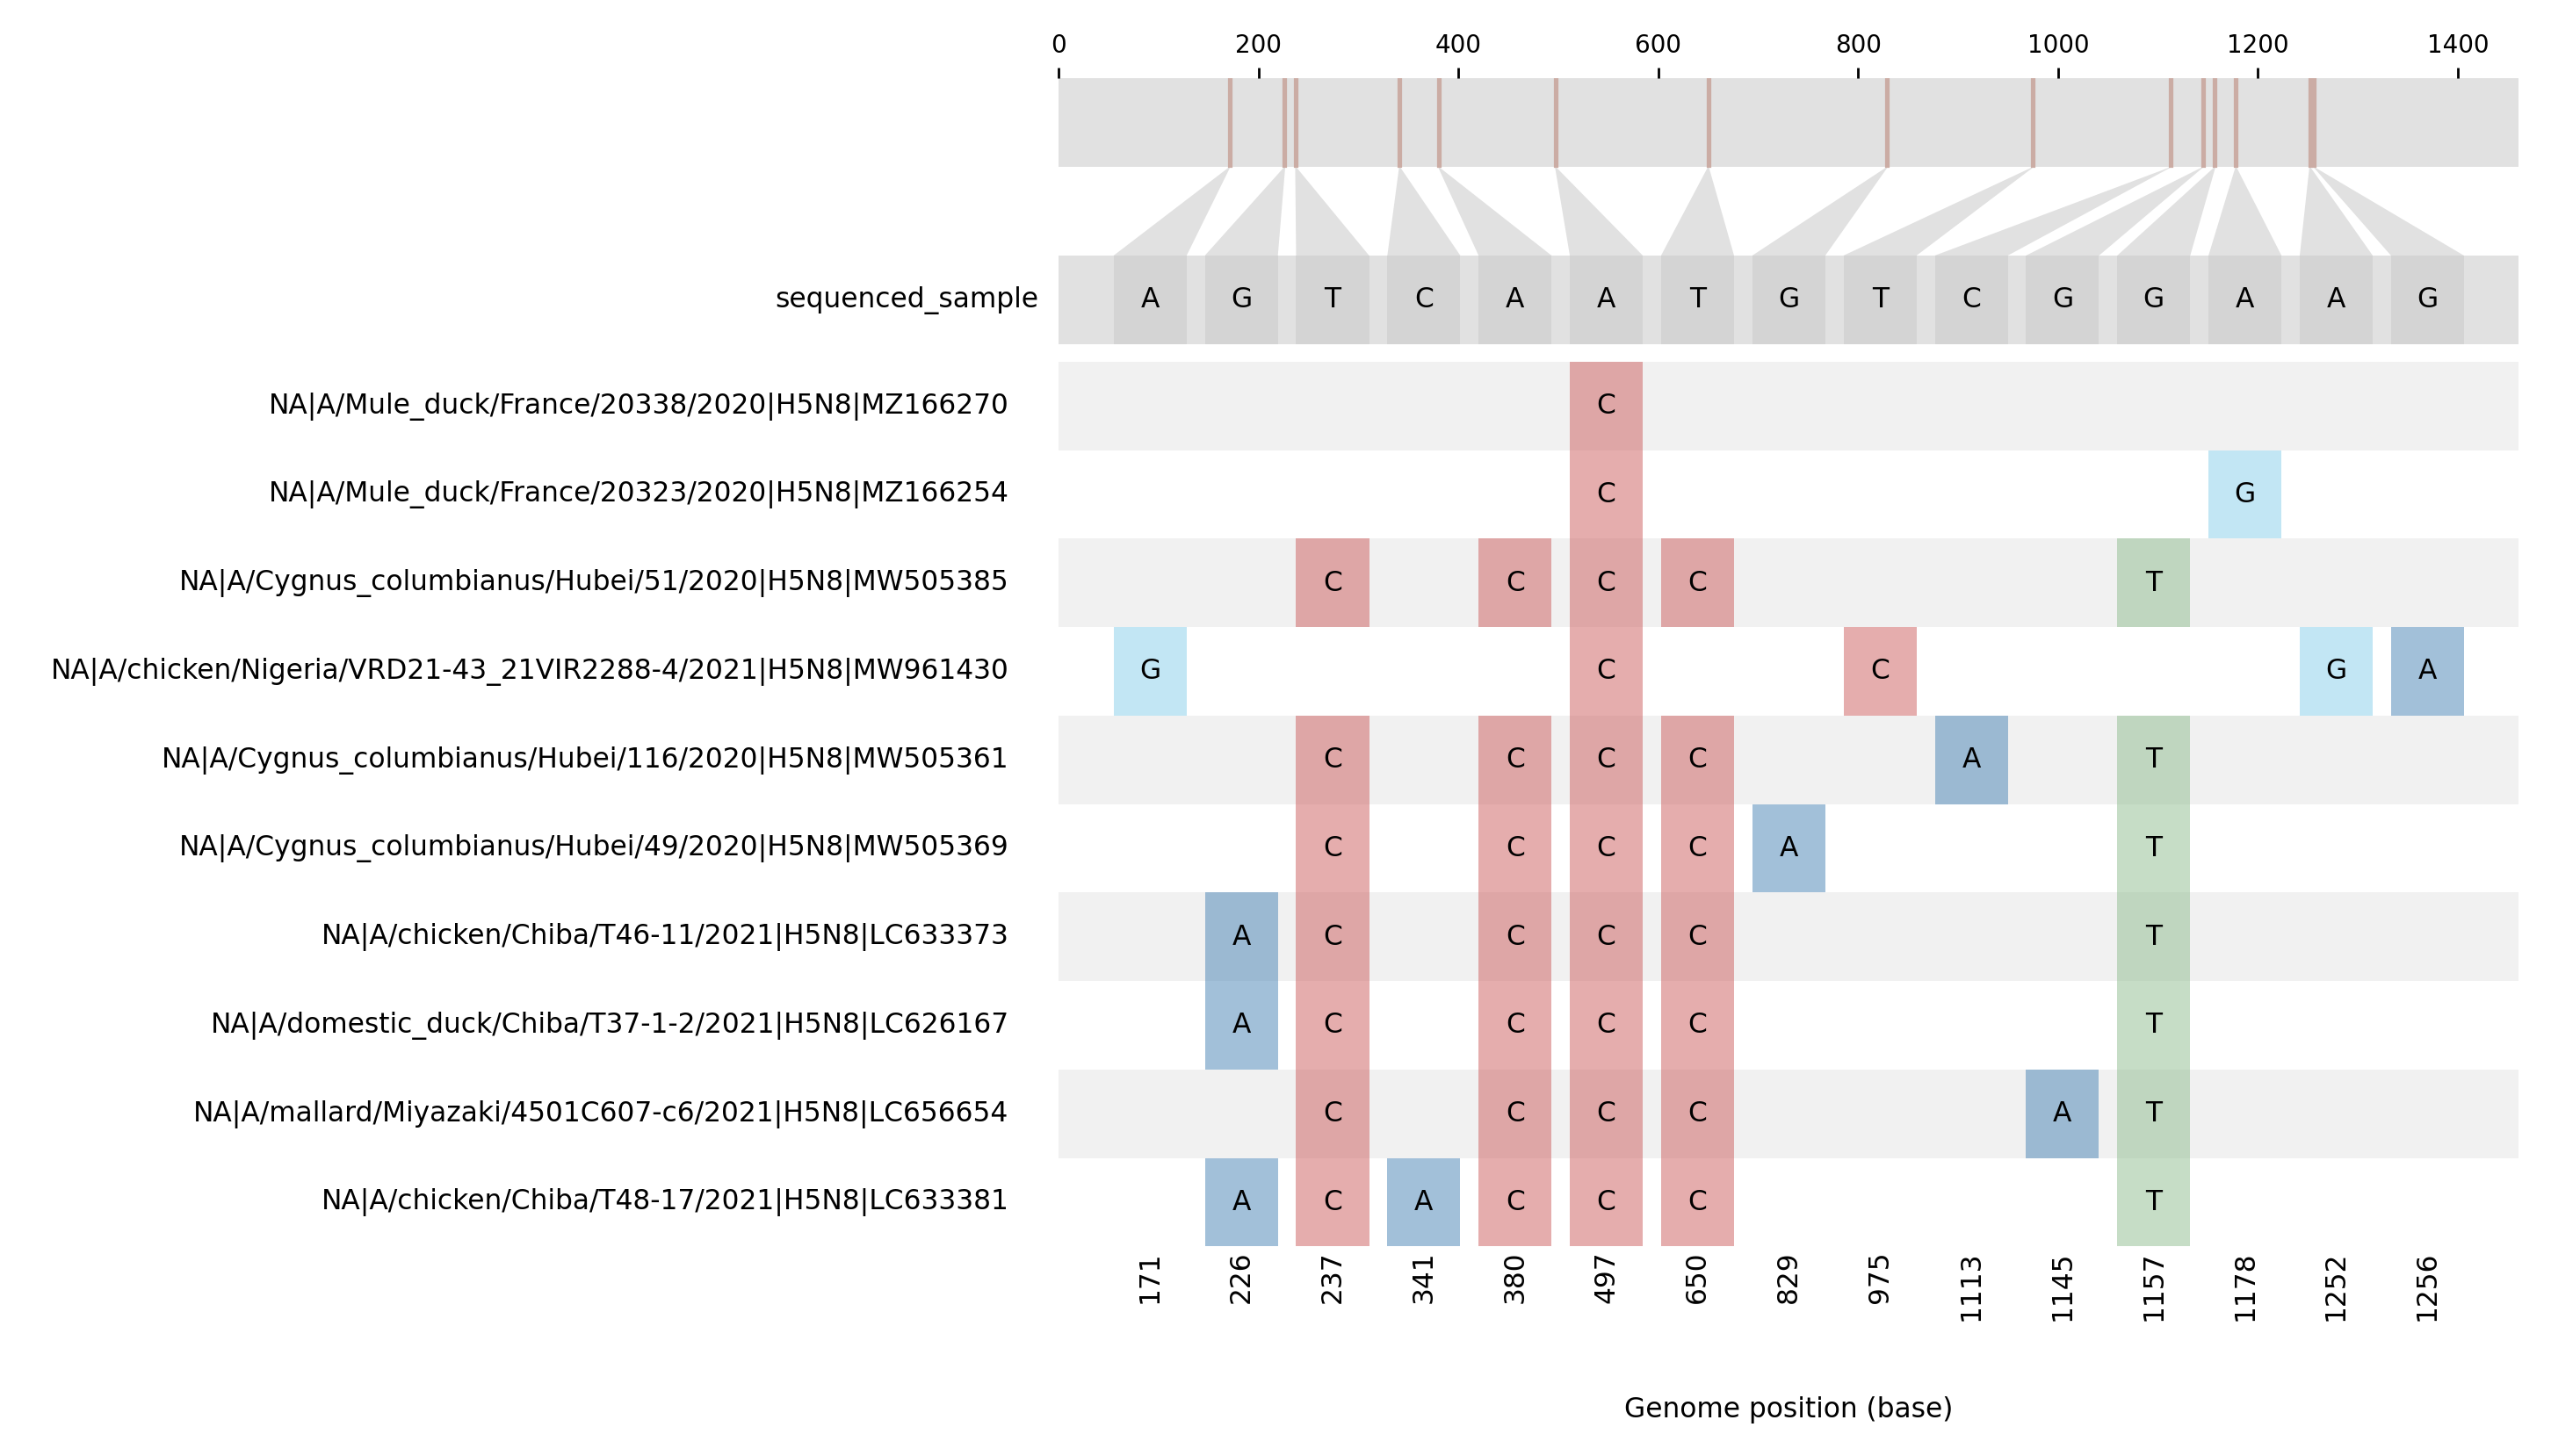
\includegraphics[width=1.0\linewidth]{media/4-aiv-snipit-s8-6-na.png}
    \caption{SNPs of NA gene of H5N8 sample.}
    \label{fig:4-aiv-snipit-s8-na}
    \end{subfigure}
    \caption[Visual summaries of SNPs in H5N8 sample.]{Visual summaries of SNPs in H5N8 sample. The consensus sequence of the gene is the reference at the top of each plot.}
\label{fig:4-aiv-snipit-s8}
\end{figure}

% todo: move to appendix?
\begin{sidewaysfigure} % todo: look that this is on an even page (read position numbers)
    \centering
    \subfloat[SNPs of HA gene of H4N6 sample.]{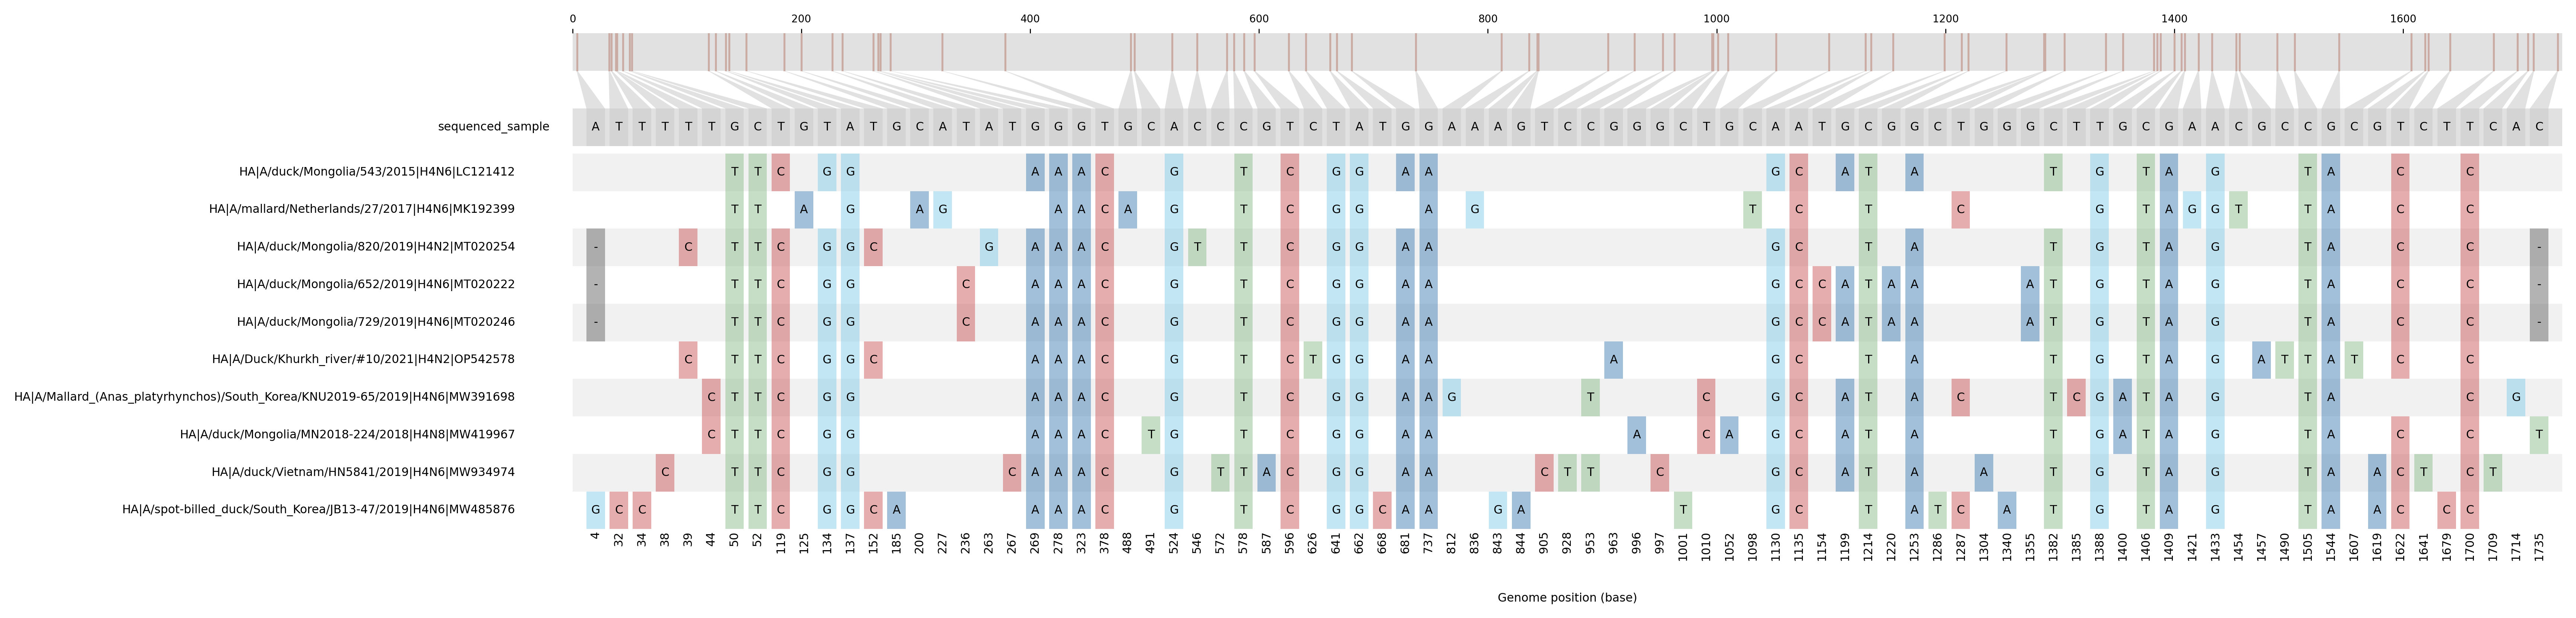
\includegraphics[width=1.0\textheight]{media/4-aiv-snipit-s4-4-ha.png}\label{fig:4-aiv-snipit-s4-ha}} \\
    \subfloat[SNPs of NA gene of H4N6 sample.]{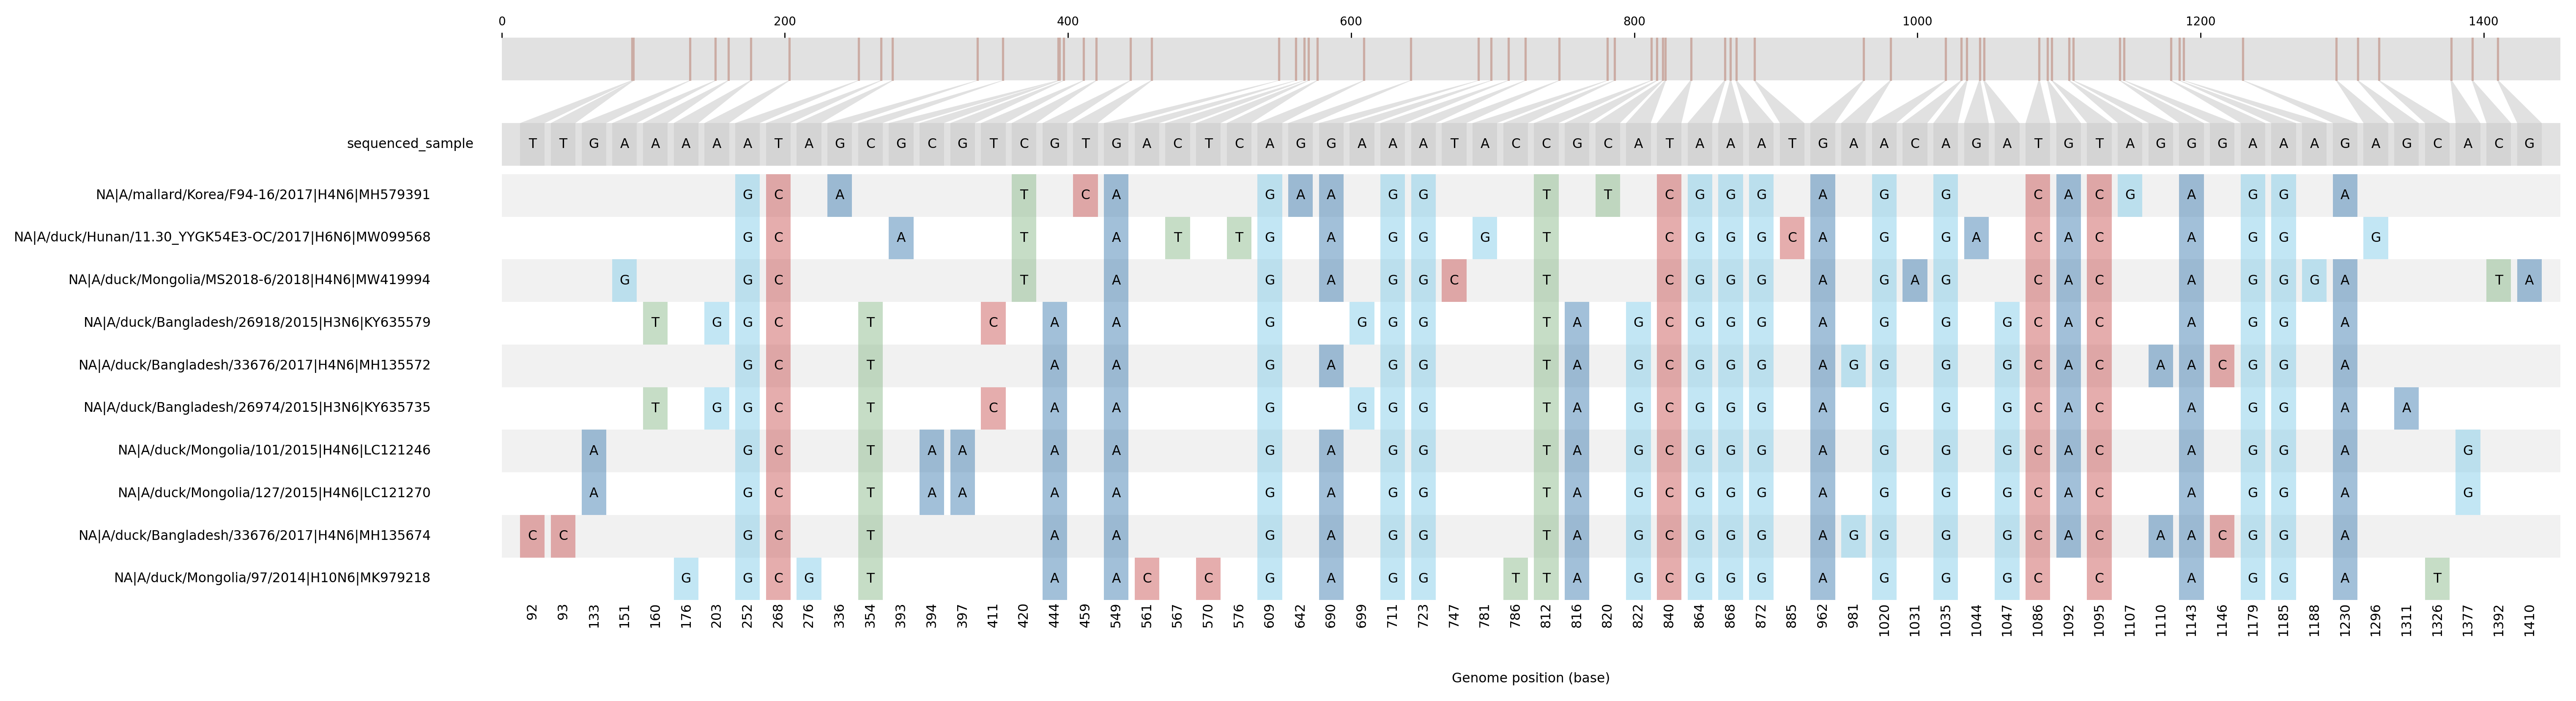
\includegraphics[width=1.0\textheight]{media/4-aiv-snipit-s4-6-na.png}\label{fig:4-aiv-snipit-s4-na}}
    \caption[Visual summaries of SNPs in H4N6 sample.]{Visual summaries of SNPs in H4N6 sample. The consensus sequence of the gene is the reference at the top of each plot.}
\label{fig:4-aiv-snipit-s4}
\end{sidewaysfigure}

\section{FMDV Workflows with Asia-1, A, SAT-1 and SAT-2 Samples}
The samples used for workflow validation are downloaded from the \ac{NCBI} and were chosen exemplatory for four of the seven different \ac{FMDV} serotypes. All four samples were sequenced on an Illumina NextSeq 550 platform. Two samples (Asia-1 serotype, SRR17960053 and A serotype, SRR18751245) were taken from infected cattle and buffalo during an outbreak in Pakistan from 2008 to 2012. One sample (SAT-1 serotype, SRR18685689) was isolated from buffaloes in Kenya in 2016 and plaque purified before sequencing, and the fourth sample (SAT-2 serotype, SRR9328470) was taken from an \ac{FMD} outbreak in Nigeria in 2014. \\
The metrics for preprocessing of the raw reads are described in~\tabref{tab:4-fmdv-metrics}. The SAT-2 sample contains a very low number of reads, however to show the ability of the developed workflows, it was kept in the test sample collection. 
\\

\setlength{\tabcolsep}{12pt}
\renewcommand{\arraystretch}{1.3}
\begin{table}[ht!]
    \centering
    \begin{tabular}{lcccc} 
    \toprule
    \textbf{Output Metric}                                                              & \textbf{Asia-1} & \textbf{A}                                           & \textbf{SAT-1} & \textbf{SAT-2}\\ \midrule
    Paired-end raw reads                                                                & 577 360         & 2 297 706                                            & 903 052        & 11 816        \\ 
    \begin{tabular}[c]{@{}l@{}}Paired-end reads after quality\\trimming\end{tabular}    & 561 280         & 2 112 856                                            & 806 712        & 11 576        \\ \midrule
    \begin{tabular}[c]{@{}l@{}}Length of assembled contigs\\with > 4000 basepairs\end{tabular} & 7 760            & \begin{tabular}[c]{@{}l@{}}12 133\\7 558\end{tabular}  & 7 329           & 7 696          \\ \bottomrule
    \end{tabular}
    \caption{Metrics after preprocessing and \textit{de novo} assembly of Asia-1, A, SAT-1 and SAT-2 serotype reads.}
    \label{tab:4-fmdv-metrics}
\end{table}

After \textit{de novo} assembly with \texttt{rnaviralSPAdes}, contigs less than half the length of the \ac{FMDV} genome size were discarded. This resulted in one contig per sample for the \ac{BLAST}n search, except for the A serotype reads, for which two contigs were assembled. As the longer contig is far larger than the \ac{FMDV} genome size, a contamination or co-infection with another virus is indicated. The \ac{BLAST}n search was performed against the \ac{NCBI} nucleotide database to identify the closest viral sequence matches. The results of the \ac{BLAST}n search showed that all the contigs were closely related to \ac{FMDV}. The highest sequence identity was observed for the Asia-1 serotype sample, with 96.74\% identity, followed by the A, SAT-1 and SAT-2 serotypes, with 94.87\%, 93.77\% and 91.42\% identity, respectively. These results were consistent with the clinical samples being positive for \ac{FMDV} infection adn the specific serotype. However, the second contig of the A sample resulted in a \ac{BLAST}n hit for pestivirus (formerly known as bovine viral diarrhea virus 1) with 93.16\% identity~\cite{smith2017proposed}. This suggests the presence of a co-infection or contamination with the pestivirus in the sample. The run with the discussed samples of this first \ac{FMDV} workflow is provided in a Galaxy history and is available via link, see Supplementary~\secref{sec:apx-fmdv-links}.

\setlength{\tabcolsep}{8pt}
\renewcommand{\arraystretch}{1.3}
\begin{table}[]
    \begin{tabular}{@{}lllll@{}}
    \toprule
    \textbf{Output Metric}                                                            & \textbf{Asia-1}    & \textbf{A}          & \textbf{SAT-1}   & \textbf{SAT-2}     \\ \midrule
    \begin{tabular}[c]{@{}l@{}}Accession no. of\\reference\end{tabular}               & KM268898.1         & JN006722.1          & KM268899.1       & JX014256.1         \\ \midrule
    \begin{tabular}[c]{@{}l@{}}Proportion of reads\\mapping to reference\end{tabular} & 100\%              & 100\%               & 100\%            & 100\%              \\
    \begin{tabular}[c]{@{}l@{}}Proportion of reference\\covered\end{tabular}          & 99.67\%            & 100\%               & 99.60\%          & 98.16\%            \\ \midrule
    Mean coverage                                                                     & 1 525.9 \texttimes & 15 895.5 \texttimes & 188.0 \texttimes & 9 302.8 \texttimes \\
    Alignment error rate                                                              & 3.47\%             & 5.08\%              & 8.18\%           & 5.87\%             \\ \bottomrule
    \end{tabular}
    \caption{Quality and coverage metrics of the alignment in the second FMDV workflow.}
\label{tab:4-fmdv-map}
\end{table}

In order to run the second workflow for reference-based mapping and consensus sequence construction for each of the four samples, the top \ac{BLAST}n hit of each sample is downloaded in FASTA format to be used as reference sequence for the respective sample. Except for the A sample, the top hit is a \ac{FMDV} genome sequence of the serotype of the query sample. In this case, user control is crucial for the selection of a plausible and representative reference sequence of the respective virus (and not the contaminating viral sequence). This is also the reason why there is no automation in the pipeline that blindly uses the top \ac{BLAST}n sequence as the reference sequence for the mapping part of the workflow.\\
This user-involving method ensures that the consensus sequence for each sample is generated based on the closest available reference sequence, which can improve the accuracy and reliability of the final assembly. Quality and coverage measures are provided for each sample are provided in~\tabref{tab:4-fmdv-map}. With the \texttt{NCBI Accession Download} tool, the plausible \ac{FMDV} sequences are downloaded to Galaxy and with \texttt{Collapse Collection} the FASTA file is extracted from the list to a single file, so that it is in a usable format for the second \ac{FMDV} workflow.\\
For each of the testing samples, the accession numbers used as references for mapping with \texttt{BWA-MEM} are listed in~\tabref{tab:4-fmdv-map}. 

\todoit
Consensus sequences:\\
- A: 3' tail: polyA, very few Ns\\
- Asia-1: 5' few Ns, first part few Ns, 3' tail few more Ns\\
- SAT-1: 5' few Ns, first part few Ns, 3' tail few more Ns\\
- SAT-2: 5' more Ns, first part more Ns, 3'  tail more Ns\\
-> relating to sequence identity and proportion of ref. covered of reference to the assembled sequence; polyC tract at 5' end

%Samples by Pirbright Institute by Dr. Graham Freimanis (NOT YET)

% \section{Workflow Profiling}
% \todoit
% Assembly vs. mapping? blast, vapor
